\documentclass[030-workshop.tex]{subfiles}

\begin{document}

    The learning materials used for the workshops can be found at
    \url{https://ds4biomed.tech/}.
    Workshop recordings are published on ``Brown Lab YouTube channel
    % TODO are footnotes allowed for stuff like this?
    \footnote{Brown Lab YouTube channel URL: \url{https://www.youtube.com/channel/UCStv5ui5yBc6_kH91h2o_qA}}
    with the ``ds4biomed'' tag.

    There were 8 workshop sessions with a total of **** registrants,
    and a total of 200 learners.

    % latex table generated in R 4.1.1 by xtable 1.8-4 package
    % Sat Oct 30 17:11:36 2021
    \begin{table}[ht]
        \centering
        \caption[Workshop Registration and Survey Counts]
            {Number of registrants, workshop attendees, and survey responses showing the amount of attrition along the way.
             More participants need to be enrolled into the study for better statistical power,
             however, that requires many more workshop iterations.
            }
        \begin{tabular}{rlllrrr}
            \hline
            & date & language & num\_registrants & num\_virtual & num\_inperson & total \\
            \hline
            1 & 2020-10-20 & r &  &  20 &  &  20 \\
            2 & 2020-10-21 & r &  &  11 &  &  11 \\
            3 & 2020-12-09 & r &  &   5 &  &   5 \\
            4 & 2021-02-02 & r &  &  19 &  &  19 \\
            5 & 2021-02-03 & r &  &  16 &  &  16 \\
            6 & 2021-05-17 & r &  &  18 &  &  18 \\
            7 & 2021-05-18 & r &  &  15 &  &  15 \\
            8 & 2021-06-29 & r &  &  10 &  18 &  28 \\
            9 & 2021-06-30 & r &  &  11 &  10 &  21 \\
            10 & 2021-09-20 & r &  &  14 &   1 &  15 \\
            11 & 2021-09-21 & r &  &   4 &   1 &   5 \\
            12 & 2021-09-22 & py &  &   9 &   2 &  11 \\
            13 & 2021-09-23 & py &  &   4 &   0 &   4 \\
            14 & 2021-09-27 & r &  &   8 &   0 &   8 \\
            15 & 2021-09-28 & r &  &   4 &   0 &   4 \\
               & Total & - & - & 168 &  32 & 200 \\
        \hline
    \end{tabular}
    \label{tab:workshop-counts}
    \end{table}

    67 responses were collected for the pre-workshop survey,
    43 responses were collected for the post-workshop survey, and
    11 responses were collected for the long-term survey.
    Across all the survey responses,
    28 respondents took a combination of the surveys.
    2 respondents took all 3 surveys,
    25 respondents took only the pre-workshop survey and post-workshop survey, and
    1 respondent took only the pre-workshop and long-term survey (Figure \ref{fig:pre-post-long-response-counts}).

    \begin{figure}[htb]
        % from 020-pre_post_long_differences.Rmd
        \centering
        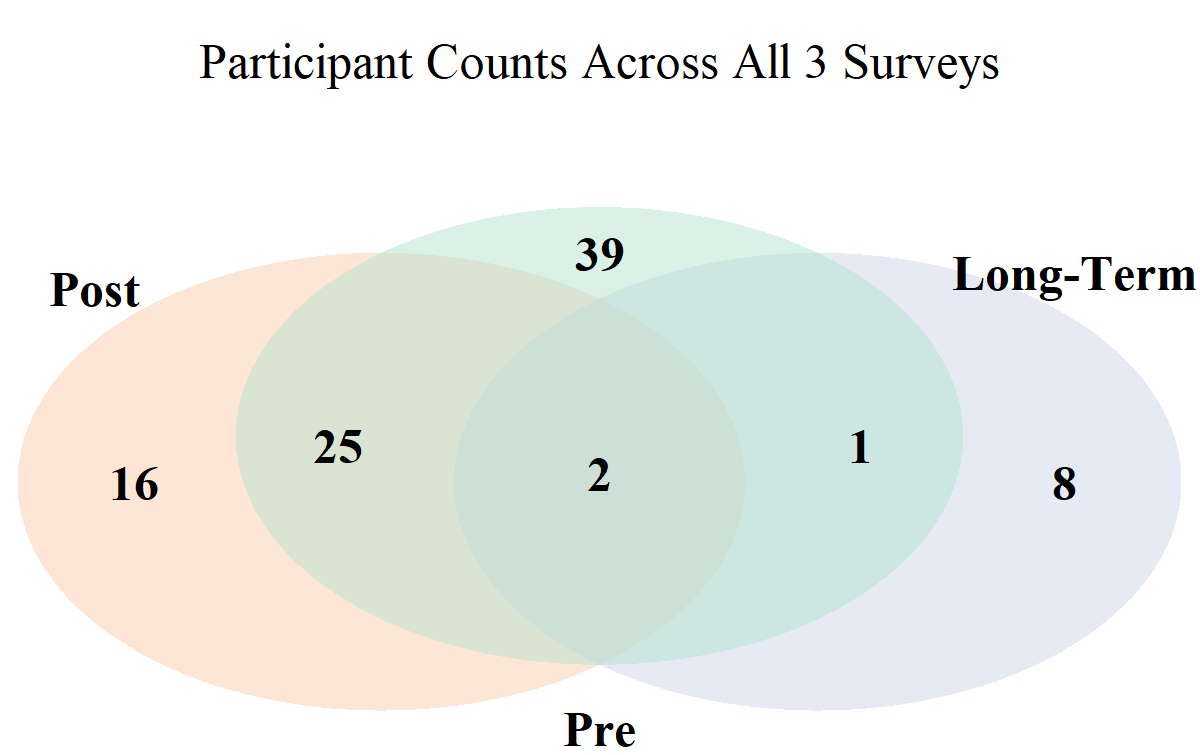
\includegraphics[]{figs/030-logitudinal/pre-post-long-response-counts}
        \caption[Response rates across all surveys (pre, post, long-term)]
        {Number of participants who responded to each of the workshop surveys:
         pre-workshop, post-workshop, and long-term workshop.
         67 responses were collected for the pre-workshop survey,
         43 responses were collected for the post-workshop survey, and
         11 responses were collected for the long-term survey.
        }
        \label{fig:pre-post-long-response-counts}
    \end{figure}

    \subsection{Create Learning Objectives}

        The learning materials were developed around 8 learning objectives:
        (1) Name the features of a tidy/clean dataset,
        (2) Transform data for analysis,
        (3) Identify when spreadsheets are useful,
        (4) Assess when a task should not be done in spreadsheet software,
        (5) Break down data processing into smaller individual (and more manageable) steps,
        (6) Construct a plot and table for exploratory data analysis,
        (7) Build a data processing pipeline that can be used in multiple programs, and
        (8) Calculate, interpret, and communicate an appropriate statistical analysis of the data.

    \subsection{Workshop Materials: ds4biomed}

        An open set of workshop materials were created, ``Data Science for the Biomedical Sciences'' (ds4biomed),
        and published with a CC0 1.0 Universal (CC0 1.0) license. % TODO cite: https://creativecommons.org/publicdomain/zero/1.0/
        At the time of writing, the book has 15 programming language agnostic chapters.
        The full table of contents is listed in Appendix \ref{ase:ds4biomed-toc}.
        The workshop teaching materials begin with basic spreadsheet concepts and
        best practices where it introduces ``tidy data'' concepts
        without using the jargon term.

        The lesson then shows how to interact with a programming language (in R or Python) using
        its respective Integrated Development Environment (IDE) and
        how to use the read-evaluate-print-loop (REPL)
        to submit code and commands to be evaluated and results printed in the console.
        The authors followed the mantra from The Carpentries of teaching the most useful tasks as early as possible
        to motivate learners.
        The first programming lesson is around loading and viewing different subsets of a
        comma-separated value (CSV) and Excel file.
        The first analysis task learners encounter is performing grouped (i.e., aggregate) statistics.
        This decision was made to also fit a conference workshop time block;
        the introduction, spreadsheets, programming, loading data, and descriptive calculation lessons
        take about 3 hours to teach.

        The next few lessons focus on data cleaning.
        The first lesson explicitly covers ``tidy data'' principles,
        how to identify common data problems,
        and how to fix them.
        This lesson walks through the ``Tidy Data'' paper published by Dr. Hadley Wickham in 2014. % TODO cite this paper here.
        And uses the more recent definition of ``Tidy Data'' from the ``R for Data Science'' book, % TODO cite book
        and illustrations by Dr. Allison Horst. % TODO cite github repo
        With an understanding of what a clean and ``tidy'' data set is,
        the next 2 lessons go through plotting and model fitting,
        which take tidy data as inputs.
        Teaching tidy data, plotting, model fitting, and conclusion also take 3 hours.

    \subsection{Longitudinal study}

        There were 3 main sets of longitudinal studies:
        (1) summary and learning objective Likert responses across all 3 surveys
        (Figure \ref{fig:pre-post-long-summary-lo})
        ,
        (2) summative assessment likert questions across just the post-workshop and long-term workhsop surveys
        (Figure \ref{fig:post-long-summative}), and
        (3) a sub-analysis looking at just summary and learning objective results from the pre-workshop and post-workshop surveys
        (Figure \ref{fig:pre-post-propprop-summary-lo} and Figure \ref{fig:pre-post-prop-summary-lo})
        .
        All any participant who took multiple surveys were dropped from the analysis.
        This was because there were not enough respondents who took all the surveys to perform a paired longitudinal analysis.
        39 responses were used for the pre-workshop study,
        16 responses were used for the post-workshop study, and
        8 resposnes were used for the long-term study (Figure \ref{fig:pre-post-long-response-counts}).

        Figure \ref{fig:pre-post-long-summary-lo} looks at each of the Likert questions in the
        summary and learning objective Likert questions across all 3 surveys.
        The overall trend is that learners have an increase in confidence across all tasks after the workshop,
        but confidence wanes off in the long-term survey.
        The same post-workshop to long-term findings applied for the summative assessment question,
        where participants were asked about their confidence to accomplish a particular data task
        (Figure (\ref{fig:post-long-summative}))

        \begin{figure}[htb]
            \centering
            \begin{subfigure}[h]{0.45\textwidth}
                \centering
                \includegraphics[scale=0.4]{figs/030-logitudinal/pre\_post\_long_summary.png}
                \caption[Pre-Post-workshop and Long-term Survey for summary likert questions]
                {Summary likert table questions}
                \label{sfig:pre-post-long-summary}
            \end{subfigure}
            \hfill
            \begin{subfigure}[h]{0.45\textwidth}
                \centering
                \includegraphics[scale=0.4]{figs/030-logitudinal/pre\_post\_long_lo.png}
                \caption[Pre-Post-workshop and Long-term Survey for learning objective likert questions]
                {Learning objective likert table questions}
                \label{sfig:pre-post-long-lo}
            \end{subfigure}
            \caption[Summary table and learning objective likert questions (pre, post, long-term)]
            {Results for 2 likert table questions in the
                pre-workshop, post-workhsop, and long-term workshop surveys.
                Results show a general increase in confidence across all questions between pre-workshop and post-workshop responses,
                and a drop in conficence across all questions between post-workshop and long-term workshop responses.
            }
            \label{fig:pre-post-long-summary-lo}
        \end{figure}

        \begin{figure}[htb]
            \centering
            \includegraphics[scale=0.4]{figs/030-logitudinal/post\_long\_summative.png}
            \caption[Summative assessment likert questions (post, long-term)]
            {Results for summative assesssment questions in the
                post-workhsop and long-term survey.
                Results show a decline in confidence to complete a particular data task.
            }
            \label{fig:post-long-summative}
        \end{figure}

        In order to make the pre-workshop and post-workshop results more comparable,
        due to varying sample sizes in each group,
        proportions of all the Likert results across the summary and learning objective questions were compared.
        The proportions of responses from the pre-workshop and post-workshop were then filled to a 100\% scale,
        to create a proportion of proportions analysis (Figure \ref{fig:pre-post-propprop-summary-lo}).
        These results show that there was a general trend to "Agree" and "Strongly Agree" to each of the Likert questions
        between the 2 longitudinal points.

        \begin{figure}[htb]
            \centering
            \begin{subfigure}[h]{0.45\textwidth}
                \centering
                \includegraphics[scale=0.4]{figs/030-logitudinal/pre\_post\_propprop\_summary.png}
                \caption[Proportion of proportions of summary Likert table results]
                {Summary likert table proportion of proportions}
                \label{sfig:pre-post-propprop-summary}
            \end{subfigure}
            \hfill
            \begin{subfigure}[h]{0.45\textwidth}
                \centering
                \includegraphics[scale=0.4]{figs/030-logitudinal/pre\_post\_propprop\_lo.png}
                \caption[Proportion of proportions of learning objective Likert table results]
                {Learning objective likert table proportion of proportions}
                \label{sfig:pre-post-propprop-lo}
            \end{subfigure}
            \caption[Summary table and learning objective likert proportion of proportions (pre, post)]
            {Results for 2 likert table questions in the
                pre-workshop and post-workhsop surveys.

            }
            \label{fig:pre-post-propprop-summary-lo}
        \end{figure}

        \subsubsection{Composite Scores}

            The responses from the Likert scale were summed together for each participant to create a composite score.
            These results confirmed the trends found in
            Figures \ref{fig:pre-post-long-summary-lo} and \ref{fig:post-long-summative}:
            learners felt more confident in the post-workshop results than the pre-workshoshop,
            and confidence waned off in the long-term survey (Figure \ref{fig:pre-post-long-composite-summary-lo}).

            \begin{figure}[htb]
                \centering
                \begin{subfigure}[h]{0.45\textwidth}
                    \centering
                    \includegraphics[scale=0.4]{figs/030-logitudinal/pre\_post\_long\_summative\_composite.png}
                    \caption[Pre-Post-workshop and Long-term Survey for summary likert composite]
                    {Summary composite likert table questions}
                    \label{sfig:pre-post-long-composite-summary}
                \end{subfigure}
                \hfill
                \begin{subfigure}[h]{0.45\textwidth}
                    \centering
                    \includegraphics[scale=0.4]{figs/030-logitudinal/pre\_post\_long\_lo\_composite.png}
                    \caption[Pre-Post-workshop and Long-term Survey for learning objective likert composite]
                    {Learning objective composite likert table questions}
                    \label{sfig:pre-post-long-composite-lo}
                \end{subfigure}
                \caption[Summary table and learning objective composite likert questions (pre, post, long-term)]
                {Taking the sum of the Likert scale results were used to create composite scores for each respondent
                 across each of the surveys.
                 In general, there was an increase in the scores from pre-workshop to post-workshop,
                 and a decline in scores from post-workshop to long-term.
                }
                \label{fig:pre-post-long-composite-summary-lo}
            \end{figure}

    \subsection{Paired Survey Responses}

    \subsection{Learning Environment}

        We know that the environment plays a critical role in a learner's ability to learn.
        There were a few instructor feedback questions in the post-workshop survey to make sure
        the presentations and learning enviornment was welcoming.
        Due to COVID-19 quarentine guidelines,
        the vast majority of workshop classes were held virtually.
        The classes that were able to be held in-person were also given virtually in a hybrid setting.

\end{document}
